In this chapter I will give an abstracted overview of the theory that is
pertinent to this thesis. In section~\ref{theory:lasercool} I will describe the
principles of laser-cooling and trapping of atoms and molecules, including
magnetic traps. In section~\ref{theory:chips} I will explain how it is possible
to create magnetic fields that will trap molecules using wires on the surface
of a chip. Next, section~\ref{theory:mols} explains the energy structure of
diatomic molecules. The chapter ends with an overview of \cm{quantum optics...}

\section{Laser-cooling and trapping}

\subsection{Doppler cooling}

We will introduce Doppler cooling in the idealised case of a two-level atom or
molecule (henceforth, the particle) travelling in one dimension.  Say that
light is incident on the particle from the positive $x$ direction. If the light
is resonant with an internal transition then the particle can absorb a photon,
which will at some later time be re-emitted and the particle will decay. The
emission of the photon has no preferred direction, and so over a large number
of these scatters the average effect is a net reduciton in the atom's velocity
in the positive $x$ direction.

In order to quantify this process, we might start by asking ourselves, what is
the force exerted on the particle by the photons? This will be~\cite{Foot2005}
%
\begin{equation}
  F = \text{photon momentum} \times \text{scattering rate}.
\end{equation}
%
The photon momentum is the usual value
%
\begin{equation}
  p_\gamma = \hbar k = \frac{hc}{\omega}
\end{equation}
%
and the scattering rate will be the product of the decay rate of the transition
(its linewidth) $\Gamma$ and the population of the excited state $\rho_{22}$.
We write the excited state in this way since it can be found from the optical
Bloch equations in the rotating wave approximation, and steady state to
be~\cite{Metcalf1999}
%
\begin{equation}
\rho_{22} = \frac{\Omega^2/4}{(\omega-\omega_0)^2 + \Omega^2/2 + \Gamma^2/4}.
\end{equation}
%
Where $\Omega$ is the Rabi frequency. We introudce the unitless parameters
$\delta = (\omega - \omega_0)/\Gamma$, $s=\Omega^2/(2\Gamma)$ so that
%
\begin{equation}
  \rho_{22} = \frac{s/2}{\delta^2 + 1 + s}.
\end{equation}
%
We can now write down the scattering rate
%
\begin{equation}
  R = \frac{s\gamma}{\delta^2 + 1 + s}
\end{equation}
%
and force follows as
%
\begin{equation}
  F = \frac{s\gamma\hbar k}{\delta^2 + 1 + s}.
\end{equation}

The force acting on the particle can be related to its velocity by the Doppler
effect. A particle moving at speed $v$ will have its resonant frequency shifted
so that it has some new frequency $\omega'$ such that
%
\begin{equation}
  \frac{\omega'-\omega_0}{\omega_0} = \frac{v}{c},
\end{equation}
%
i.e.\ the frequency is red-detuned from the transition frequency at rest. The
result is that $\delta$ can be re-written as
%
\begin{equation}
  \delta \rightarrow \delta_+ = \delta + \frac{\omega_0}{\gamma c}v
\end{equation}
%
where $\delta$ represents the detuning of the laser from the resonant frequency
at rest, and the second term is the additional shift due to the Doppler effect.

However, what if the light is incident from the negative $x$ direction? In this
case, there is a blue not a red shift, and we have
%
\begin{equation}
  \delta \rightarrow \delta_- = \delta - \frac{\omega_0}{\gamma c}v.
\end{equation}
%
By combining counter-propagating beams, it is possible to create a net force
%
\begin{equation}
  F_\text{res} = F_+ + F_-
\end{equation}
%
where
%
\begin{equation}
  F_\pm = \frac{s\gamma\hbar k}{\delta_\pm^2 + 1 + s}.
\end{equation}
%
For small $v$ we perform a Taylor expansion around $v=0$ to find that
%
\begin{equation}
  F_\text{res} \approx \frac{4\hbar k^2 s \delta}{(1 + s
  +\delta^2)^2}v.
\end{equation}
%
Which is maximised when $\delta = -1$ and $s = 1 + \delta^2 = 2$, so that
%
\begin{equation}
  F = -\frac{\hbar k^2}{2} v = - \alpha v.
\end{equation}
%
So the counter-propagating beams provide a velocity-dependent damping
force. We call this arrangement an optical molasses, and it can equally be
applied in three dimensions.

It is important to note that the particles will not be brought to a standstill
under this effect. The molasses force does not contain the information
on the heating that occurs when the particles re-emit the absorbed photons.
This stochastic process limits the minimum attainable temperature to the
Doppler temperature~\cite{}
%
\begin{equation}
  T_D = \frac{\hbar\Gamma}{k_B}.
\end{equation}

\subsection{Magneto-optical trap}

Doppler cooling is an important tool in the creation of ultracold atoms and
molecules, but it is of note that this technique does not provide any
position-dependent restoring force, i.e. molecules that are slowed by the
above-described techniques are not trapped.
%
The magneto-optical trap (MOT) is the preeminent tool of atomic and molecular
physics, providing a way to trap a relatively cold gas of particles. It is the
backbone of many experiments~\cite{} including our own~\cite{}. In this section
I will describe the basic operation of the common type-I MOT, that is a two
level system where the the ground state has angular momentum $F=0$ and the
excited state has angular momentum $F'=1$.  In reality the molecule MOTs that
we will discuss are type-II systems ($F'\leq F$) but these are more complicated
and will be discussed in section~\ref{section:overview}.

The MOT consists of two components, a magnetic quadrupole field, and restoring
laser beams, which are detuned from the $F\rightarrow F'$ transition by some
amount $\delta$. This setup is shown for one dimension in \cm{fig from
presentation}. The Zeeman effect lifts the degeneracy of the excited state, and
introudces the usual energy shift~\cite{Binney}
%
\begin{equation}
  \Delta E = g_F m_F \mu_B B
  \label{theory:eqn:zeeman}
\end{equation}
%
where $g_F$ is the Land\'e g-factor, $\mu_B$ is the Bohr magneton, and $B$ is
the magnetic field. For a one-dimensional quadrupole field, we write $B=B'x$,
where $B'$ is the field gradient. We therefore have a position-dependent change
in the energy. Note that for negative $x$, the $m_F=-1$ state has lower energy,
and for positive $x$ the $m_F=1$ state has lower energy (when $g_F>0$, if
$g_F<0$ this is reversed).
%
The detuning $\delta$ is chosen such that this shift brings the lowered state
into resonance with the light, meaning that the particle will preferrentially
absorb photons when it is away from the centre.

\begin{figure}[ht]
  \centering
  \includegraphics[width=0.8\textwidth]{figs/theory/motThesis.pdf}
  \caption{Illustration of the operating principle of a one-dimensional MOT on
    a two-level system with $F=0$ and $F'=1$. The particle is represented by
    the circle, and has counter-propagating beams of light (pink arrows)
    incident on it. A quardupole magnetic field is applied, lifting the
    degeneracy of the excited state as shown by the black lines. The light is
    red-detuned so as to be resonant with the transition to the lower $m_F$
    state, but only the restoring beam will be absorbed due to the choice of
    polarisation. The excited state will decay back to the ground state (dashed
    lines).
  }
  \label{theory:fig:MOT}
\end{figure}

We wish to ensure that when a photon is absorbed the momentum change provides a
restoring force towards the centre of the MOT. This is achieved by choosing the
polarisation of the light so that coming from the positive (negative) $x$
direction, the light has $\sigma^+$ ($\sigma^-$) polarisation. The result is
that the particle will then always absorb light that is propagating towards the
centre of the trap, resulting in a restoring force. We also observe the same
Doppler cooling force from the molasses, so the resulting force is
% TODO CITE, this is from Ed's notes
%
\begin{equation}
  F = - \alpha v - \left(\frac{\mu B'}{\hbar k}\right)\alpha x.
\end{equation}

\subsection{Sub-Doppler cooling}

We might expect that a MOT would cool the atoms to around the Doppler
temperature, but in fact the temperate reached is often lower, due to
sub-Doppler cooling effects that often occur in a MOT. Chiefly, we consider
polarisation gradient cooling. This cannot occur in the $F=0$, $F'=1$ system
used to introduce the MOT, so we consider instead a new system with $F=1/2$,
$F'=3/2$ which we note is still a type-I MOT.

In the centre of the MOT where there is near zero magnetic field, the $m_F$
states of the system would be degenerate expect that the degeneracy can be
lifted by the field of the light. This is the a.c. Stark shift, which is a
function of the polarisation of the light. When the light has $\sigma_\pm$
polarisation, the $m_F=\mp1/2$ state is mixed more strongly with the exited
state, and so is higher. The relative matrix elements are shown in \cm{fig to
reproduce from Ed or elsewhere...}.

\begin{figure}[htb]
  \centering
  \begin{subfigure}[b]{0.45\textwidth}
      \cm{Optical pumping fig}
    \end{subfigure}
  \begin{subfigure}[b]{0.45\textwidth}
    \begin{overpic}[width=0.8\textwidth]{figs/theory/molasses.pdf}
      \put(4, 50){(b)}
      \put(105, 60){$F'=3/2$}
      \put(105, 28){$F=1/2$}
      \put(105, 2){Polarisation}
    \end{overpic}
    \end{subfigure}
    \caption{In (a) we have \cm{some coupling matrix elements} Subfigure (b)
      shows the polarisation gradient cooling scheme described in the main
      text.  The polarisation gradient is depicted in the bottom row, and the
      $m_F=1/2$ ($m_F=-1/2$) state is shown by the dashed (solid) line. A
      particle in the molasses (pink circle) will follow a path such as the one
      shown here in pink, being pumped into the $F'=3/2$ state at the top of
      the potential hill, then decaying (dashed grey lines) back to the lower
      of the ground states and climbing the hill again. \cm{Cite inspiration}
  }
\end{figure}

The counter-propagating beams establish a polarisation gradient across the
trap, and hence the Stark shift of the ground states also varies across the
trap, as shown in \myfigref{}. We have the additional effect that the
$m_F=\pm1/2$ state is only pumped by the $\sigma^\mp$ light, and so it happens
that the state with higher energy is the one that is excited. The excited state
can decay into the lower of the two ground states, where it will follow the
potential curve until it is pumped again. The particles on average spend more
time climbing the potential than descending it, and therefore expend energy
through this process, reducing their temperature to \cm{the recoil limit?}

\cm{TODO: what is the minimum temp?}

\cm{Also possible to just have the molasses, no B field and then we have
  sub-Doppler cooling}

\subsection{Magnetic trapping}

% TODO want to cite 2d mots, pyramid mots, grating mots, etc.
The MOT is an important tool for trapping, and can be configured in various
ways~\cite{}, but there is considerable benefit to being able to confine
particles using only a magnetic field. Since there is no light involved, it is
much easier to control the trapping potential. This opens the door to
applications in guiding~\cite{} and transporting~\cite{} particles, but also of
course, confining close to a surface. This will be discussed in more detail in
the next section, but for the moment we lmit ourselves to a basic description
of magnetic trapping.

Continuing with the above example of a two-level particle with $F=1/2$,
$F'=3/2$, we notice that when the particle is in a state where $g_F m_F > 0$,
the Zeeman shift due to a magnetic field is positive (c.f.\
\myeqref{theory:eqn:zeeman}). Hence if the magnetic field $B$ is chosen such
that there is a local minimum in the vicinity of the particle, then these
states will be attracted to that minimum. Such a state is called a weak-field
seeker. We can equally have stong-field seeksers when $g_F m_F < 0$, but these
cannot be trapped since it is not possible to create a local magnetic field
maximum in free space.
%
Note that the dependence here is on the magnitude of the magnetic field, so the
direction of the field does not directly affect the trapping potential.

So to magnetically trap our particle we need to first ensure it is in a
weak-field seeking state, and then we need to introduce a magnetic field with a
local minimum. It is possible to transfer into either of the states
$\ket{F=3/2, m_F=\pm3/2}$, applying only $\sigma_\pm$ light will optically pump
into the respective state. After the pumping scheme it is possible (if desired)
to either of the $\ket{F=1/2, m_F=\pm1/2}$ states by a \cm{microwave
transition}. Depending on the sign of $g_F$ (or for the excited state $g_{F'}$) 
one of these states is bound to be a weak-field seeker.

Now the final ingredient is a magnetic potential with a local minimum. There
are a plethora of examples to choose from, but the canonical choice is the
quadrupole trap, which can be fomred from a pair of anti-Helmholtz coils, as
shown in \mysubfigref{theory:fig:fields}{a}. We can approximate the field
generated near the centre of such a configuration as~\cite{} % Metcalf?
%
% TODO I use this equation somewhere else and I need to change to reference
% this one...
\begin{equation}
  \mathbf{B} = B'\begin{pmatrix} -x/2 \\ -y/2 \\ z \end{pmatrix}
  \label{theory:eqn:quadrupole}
\end{equation}
%
where $B'$ is the field gradient in the $z$ direction, and depends on the
currents in the coils as well as their geometry.

\begin{figure}
  \centering
  \includegraphics[width=0.7\textwidth]{figs/theory/QPIP.pdf}
  \caption{Subfigure (a) demonstrates the generation of a quadrupole field
    (pink arrows) by
  anti-Helmholtz coils (black arrows). Subfigure(b) demonstrates the current
  configuration for a
  Ioffe-Pritchard trap, with longitudinal currents (blue arrows) and endcap
coils (black arrows) The field near the trap centre is also shown (pink arrow).
\cm{reproduced from Ed's notes}}
  \label{theory:fig:fields}
\end{figure}

One of the drawbacks to a qaudrupole is taht the magnetic field at the centre
is zero. In regions of low field there is no breaking of the degeneracy, and so
it is possible for the $m_F$ quantum number to change to an un-trappable state.
This is known as a spin-flip or Majorana loss.~\cite{} One method of resolving
this is to instead use a Ioffe-Pritchard trap, which has a non-zero field
minimum. The standard method of implementing such a trap is shown in
\mysubfigref{theory:fig:fields}{b}. Four straight wires are arranged in a
square, with a pair of parallel coils on either end to form end-caps. The field
generated is of the form~\cite{} % Metcalf?
%
\begin{equation}
  \mathbf{B} = b_1 \begin{pmatrix} x \\ -y \\ 0 \end{pmatrix}
  + b_0 \begin{pmatrix} 0 \\ 0 \\ 1 \end{pmatrix}
  + b_2 \begin{pmatrix} -xz \\ -yz \\ z^2 - \rho^2/2 \end{pmatrix}
  \label{theory:eqn:IP}
\end{equation}
%
where $\rho^2 = x^2 + y^2$ and the constants $b_i$ are again functions
of the currents and the geometry.

For a quadrupole field, the motion is characterised by the gradient, but for a
Ioffe-Pritchard trap, the motion is harmonic, and we can find the frequencies
by evaluating the shape of the potential $\mu B$, where $\mu$ is the magnetic
moment of the trapped state. From \myeqref{theory:eqn:IP} we have
%
\begin{equation}
  \mu B \approx \mu \sqrt{b_0^2 + (b_1^2 -
  b_0b_2)\rho^2 + 2b_0b_2z^2}.
\end{equation}
%
Up to the third order in position terms. Now expanding for $z=0$ and small $\rho$ we get
%
\begin{equation}
  \mu B \approx \mu b_0\left(1 + \frac{b_1^2 -
    b_0b_2}{2b_0}\rho^2\right)
\end{equation}
%
which is a harmonic potential with minimum $\mu b_0$ and frequency
%
\begin{equation}
  \omega_\rho = \sqrt{\frac{\mu}{m}\left(\frac{b_1^2}{b_0}-b_2\right)}
\end{equation}
%
for a particle of mass $m$.

Similarly for the $z$ direction, we can find the potential
approximates to
%
\begin{equation}
  \mu B = \mu b_0 (1 + b_2 z^2)
\end{equation}
%
which is again harmonic, with frequency
%
\begin{equation}
  \omega_z \approx \sqrt{\frac{\mu}{m}2b_2}.
\end{equation}

% TODO Cite, could do Treutlein but would rather not (this was foriginally from
% Ed's notes)

We note that the motion of the particles in the trap must be slow compared to
the resonant frequency $g_F\mu_BB/\hbar$ to avoid inducing transitions.
Similarly, the field can be changed adiabatically (slowly compared to the speed
of the trapped particles) without heating~\cite{}. This can be used for
transport, or transferring particles between magnetic traps, and will be
discussed further in chapter~\ref{sim}.

\section{Chip trap theory}
\label{theory:chips}

Of course, the main subject of this thesis is the trapping of particles near
chips. In this section we will see that it is possible to use wires on a chip,
combined with external magnetic fields to produce trapping potentials that
resemble either a quadrupole or Ioffe-Pritchard trap.

\subsection{Simple wire traps}

We begin our discussion by considering a simple case of a two-dimensional trap.
This will be formed of a straight wire carrying current $I$, which we
approximate to have infinite length. Such a wire can be free-standing or
deposited on a substrate. The magnetic field due to the wire is described by
the Biot-Savart law~\cite{}, having magnitude
%
\begin{equation}
  B_w(r) = \frac{\mu_0 I}{2 \pi r}
\end{equation}
%
$r$ is the distance from the wire. The direction of the field obeys the right
hand rule. With such a geometry it is possible to create a ruidmentary
two-dimensional trap at a distance $h$ from the wire, by applying an external
bias field, whose direction opposes the field of the wire. To create the trap
at the desired bias, the strength of the field must be $\tilde{B}_y =
B(h)$~\cite{2011Ac}.

%TODO Use this notation in sim when descirbing calculation of the field!
Figure \myfigref{theory:fig:simplefield} illustrates this two-dimensional trap.
Here the wire oriented along the $x$ direction, with the current
$I=\SI{1}{\milli\ampere}$, flowing in the
positive direction (out of the page). This generates the expected field
$\mathbf{B}$ shown in subfigure (a). This is superimposed with the bias field
$\mathbf{\tilde{B}}_y$, also shown in (a), to produce the resulting field
$\mathbf{B} = \mathbf{B}_w + \mathbf{\tilde{B}}$ shown
in (b). This subfigure details the field lines (pink arrows), however these do
not tell the whole story, since weak-field seekers go to areas where the
magnitude of the field ($B$) is low. This is shown by the gradient, with darker
areas (blue, guide to the eye) indicating areas of lower field. The bias field
is chosen to induce a field minimum at $h=\SI{1}{\milli\meter}$. Subfigure (c)
shows a cut-through of the potential along $y$ with $x=0$, $z=h$. Subfigure (d)
also shows a cut-through of the potential along $z$ with $x=y=0$. This
demonstrates the two-dimensional trap.

\begin{figure}[htbp]
  \centering
  \begin{subfigure}[b]{0.45\textwidth}
    \centering
    \hfill{}
    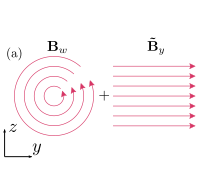
\includegraphics[width=0.8\textwidth]{figs/theory/wires/simplefield.pdf}
    \hfill{}
  \end{subfigure}
  \begin{subfigure}[b]{0.45\textwidth}
    \centering
    \import{figs/theory/wires/}{simpleheat_alone.pgf}
  \end{subfigure} \\
  \begin{subfigure}[b]{0.45\textwidth}
    \centering
    \import{figs/theory/wires/}{simpleheat_y.pgf}
  \end{subfigure}
  \begin{subfigure}[b]{0.45\textwidth}
    \centering
    \import{figs/theory/wires/}{simpleheat_z.pgf}
  \end{subfigure}
  \caption{
    The field from a simple two-dimensional wire trap. In subfigure (a) a wire carries
    current $I=\SI{1}{\milli\ampere}$ in the positive $x$ direction (out of the
    page) to create the usual field $\mathbf{B}_w$. This is combined with the
    external bias field $\mathbf{\tilde{B}}_y$ to create the two-dimensional trap
    at height $h=\SI{1}{\milli\meter}$
    shown in subfigure (b). The field lines are shown by pink arrows, and the
    magnitude of the resulting field is shown with the blue gradient (darker
    means weaker field, guide to the eye). Cut throughs of the potential are
    shown for $y$ (with $x=0$, $z=h$) in (c) and for $z$ (with $x = y = 0$) in
    (d).
  }
  \label{theory:fig:simplefield}
\end{figure}

Since the field minimum here is a zero, we can approximate the value near the
centre by a (two-dimensional) quadrupole with gradient
%
\begin{equation}
  B' = -\frac{2\pi \tilde{B}_y^2}{\mu_0 I}.
\end{equation}
%
The depth of the trap is $\mu \tilde{B}_y$, where $\mu$ is the \cm{magnetic dipole
moment} of the trapped particle. This can be seen in
\mysubfigref{theory:fig:simplefield}{d}: the potential is $B = |B_w(z) +
\tilde{B}_y|$, and so has an asymptote at $B=|\tilde{B}_y|$ as
$z\rightarrow\infty$.
%
We can transform such a trap into a Ioffe-Pritchard trap by applying a second
bias field along the $x$ direction to lift the field minimum away from
zero~\cite{2011Ac}.

Of course, it is commonly desirable to trap in all three dimensions. A simple
way to introduce confinement along the $x$ axis is to introduce a secocond wire
trap acting in the perpendicular direction. Such a device is called a dimple
trap (or cross conductor trap, or X-trap) and is illustrated in
\myfigref{theory:fig:dimple}. We label the current in the second wire $I_1$
and the new bias field, which is parallel to the $x$-axis and opposes the
$I_1$ field is labelled $\mathbf{B}_x$. In the case that $I_1 \ll I$, the
second wire can be treated as a perturbation of the first. The field minimum is
therefore still at $h$, and its depth is \cm{ref earlier equation?}.

\begin{figure}[htb]
    \centering
    \begin{tabular}[t]{cc}
\begin{subfigure}{0.3\textwidth}
    \centering
    \smallskip
    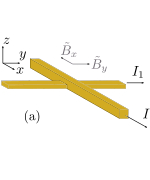
\includegraphics[width=\textwidth]{figs/theory/wires/dimple.pdf}
\end{subfigure}
    &
        \begin{tabular}{c}% if you add [t], than sub images are pushed down
        \smallskip
            \begin{subfigure}[t]{0.4\textwidth}
                \centering
                  \import{figs/theory/wires/}{dimpleheat_alone.pgf}
            \end{subfigure}\\
            \begin{subfigure}[t]{0.4\textwidth}
                \centering
                  \import{figs/theory/wires/}{dimple_x.pgf}
            \end{subfigure}
        \end{tabular}\\
    \end{tabular}
  \caption{
    The geometry of the dimple trap is shown in subfigure (a), with the new
    wire along $y$ carrying current $I_1$ intersecting the $I$ wire. An
    additional bias field in the $x$ direction, $\tilde{B}_x$ creates the field
    minimum. The field lines (pink) and magnitude (blue, darker is weaker,
    guide to the eye) is shown in subfigure (b) along $x=0$. Note the strong
    field region along the $y$ axis around the $I_1$ wire. Subfigure (c) shows
    a cut-through of the trapping potential in the $x$ direction with $y=0$,
    $z=h$.
  }
  \label{theory:fig:dimple}
\end{figure}

The dimple trap can be used as a quadrupole trap when the bias fields are
chosen to exactly cancel the magnetic field at the centre, or it can be used as
a Ioffe-Pritchard trap when there is a non-zero minimum. We will focus on the
latter case, in which case it is useful to write down the trap frequencies, the
derivation of which is similar to the one for the six-wire field discussed in
\cm{ref theory to be writtern}.
Since the trapping from the $I$ wire will be stronger than the $x$-axis
confinement from the $I_1 << I$ wire, we $\omega_x$ to be the weak trapping
direction. We again write down the field minimum
%
\begin{equation}
  B_0 = \left|\tilde{B}_x + \frac{\mu_0 I_1}{2\pi h}\right|,
\end{equation}
%
the transverse gradient
%
\begin{equation}
  B'_\perp = \frac{\mu_0 I}{2 \pi h^2},
\end{equation}
%
and the curvature along the weak component
%
\begin{equation}
  B'' = \frac{\mu I_1}{\pi h^3}.
\end{equation}
%
The trap frequency in the strong direction is~\cite{2011Ac}
%
\begin{equation}
  \omega_\perp = \sqrt{\frac{\mu B_\perp'^2}{m B_0}}
  \label{theory:eqn:perpfreq}
\end{equation}
%
where $m$ is the particle mass. In the weak direction (along $x$) the frequency
is~\cite{2011Ac}
%
\begin{equation}
  \omega_x = \sqrt{\frac{\mu B''}{m}}.
  \label{theory:eqn:xfreq}
\end{equation}

\subsection{The H-trap}

Consider the dimple trap, but with $\tilde{B}_x$ set to zero. Now what was
previously a magnetic field minimum will be a field maximum. By putting two
such dimple traps next to each other, it is possible to create a local minimum
within which we can trap molecules. Such a trap is called an H-trap, and is
pictured in \myfigref{theory:fig:Htrap}. We label the current due to the second
dimple trap $I_2$, and again note that the bias field in the $x$ direction can
be set to zero. The distance between $I_1$ and $I_2$ is denoted $d$, and we now
refer to the wire carrying current $I$ as the axis of the trap.

\begin{figure}[htb]
  \centering
  \begin{subfigure}[b]{0.4\textwidth}
    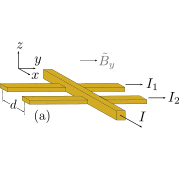
\includegraphics[width=\textwidth]{figs/theory/wires/Htrap.pdf}
    %\vspace{0.1mm}
  \end{subfigure}
  \begin{subfigure}[b]{0.4\textwidth}
    \import{figs/theory/wires/}{Hx.pgf}
  \end{subfigure}
  \caption{The geometry of the H-trap is shown in subfigure (a). In subfigure
  (b) we show the potential for an H-trap with
  $I_1=I_2=I/10=\SI{0.1}{\milli\ampere}$ and $d=\SI{10}{\milli\meter}$. Again the bias field is chosen so
  that $h=\SI{1}{\milli\meter}$.}
  \label{theory:fig:Htrap}
\end{figure}

We note that we need not choose $I_1$ and $I_2$ to be the same, although from
now on we will assume that they have the same magnitude, the sign can differ.
In other words the currents can be parallel or anti-parallel. In the former
case the trap forms a Ioffe-Pritchard trap; this is due to the fields from
$I_1$ and $I_2$ adding in the centre, to provide some overall non-zero
component in the $x$ direction. When the currents are anti-paraellel, the $I_1$
field opposes the $I_2$ field in the centre of the trap, the two cancel and
there is a field zero. Hence the latter configuration is a quadrupole trap.

In the Ioffe-Pritchard configuration, we can write down the field's
minimum~\cite{PhysRevA.79.013407}
%
\begin{equation}
  B_0 = \tilde{B}_x + 2\tilde{B}_y \frac{I_1}{I}\frac{h^2}{(d/2)^2 + h^2}
\end{equation}
%
transverse gradient~\cite{PhysRevA.79.013407}
%
\begin{equation}
  B'_\perp = \frac{2\pi\tilde{B}_y}{\mu_0 I}
\end{equation}
%
and curvature (in the $h \ll d$ limit)~\cite{PhysRevA.79.013407}
%
\begin{equation}
  B'' = \frac{12\tilde{B}_y I_1 h^2}{I (d/2)^4}
\end{equation}
%
and the trap frequencies are again given by equations~\ref{theory:eqn:perpfreq}
and~\ref{theory:eqn:xfreq}. In the quadrupole configuration, the traps is
characterised by the perpendicular gradient $B'_\perp$. 

\subsection{Three dimensinal single-wire traps}

Although the H-trap provides a method of creating a three dimensional
microtrap, it is not always convenient to have to use three distinct wires.
Fortunately the H-trap can be approximated by a single wire, either in a
U-shape for the quadrupole variant, or a Z-shape for the Ioffe-Pritchard
variant. These are pictured in \cm{theory:fig:HUZ}. Note that for the U-trap
the currents in the off-axis wires are once again anti-parallel, and in the
Z-trap these currents are parallel. For the U- and Z-traps, we denote the
distance between the end wires as $d$, and again refer to this as the axis.

\begin{figure}[htbp]
  \centering
  
\includegraphics[width=\textwidth]{figs/theory/wires/HUZcomp.pdf}
  \caption{Current configuration for U-trap (Z-trap) approximating the
  quadrupole (Ioffe-Pritchard) H-trap configuration.}
  \label{theory:fig:HUZ}
\end{figure}

The Z-trap will be the primary focus of this thesis, and so we will focus on
this as an example. In \myfigref{theory:fig:HZcontours} we compare an H-trap
with a current of \SI{1}{\milli\ampere} on each wire with the potential due to
a single Z-wire also with current \SI{1}{\milli\ampere}. In both cases
$d=\SI{10}{\milli\meter}$, and a bias field of \SI{2}{\milli\gauss} in the $y$
direction is chosen, so as to create a minimum at approximately
$z=\SI{1}{\milli\meter}$ from the axis. The potentials are similarily
comparable for the H-trap in quadrupole configuration and the U-trap.

\begin{figure}[htbp]
  \centering
  \import{figs/theory/wires/}{HZcontours.pgf}
  \caption{Contour plots comparing the potentials for a H-trap in
    Ioffe-Pritchard configuration (left column) and Z-trap (right column), with
    cut throughs for $z=\SI{1}{\milli\meter}$ (top row) and $x=0$ (bottom row).
    All wires carry a current of $I=\SI{1}{\milli\ampere}$ and a bias field of
    \SI{2}{\milli\gauss} is applied in the $y$ direction.}
  \label{theory:fig:HZcontours}
\end{figure}

This illustrates that a single current-carrying wire can be used to form a trap
in three dimensions. The examples here use length scales of a few millimeters,
and have typical depths of \cm{??}, but we will discuss in chapter~\ref{sim}
that it is possible to realise much smaller trap and \cm{deeper} traps.


\section{Diatomic molecule theory}
\label{theory:molecules}

Up to this point we have considered abstracted and idealised systems, but in
the next chapter we will begin to think about the realities of implementing a
cold molecule experiment. It is essential that we introduce and understand the
energy structure of diatomic molecules, which is far richer and more complex
than the structure of atoms, due to the additional effects of vibration and
rotation of the two nuclei.

\subsection{Electronic, vibrational, and rotational energy}

We can begin by considering two atoms or ions, which we label $A$ and $B$,
with masses  $m_i = m_p Z_i$, $i\in\{A,B\}$ and $m_p$ is the proton rest mass. We say that the location of the
atoms is $\mathbf{R}_i$ and the distance between them is
$R_{AB}$ where $\mathbf{R}_{AB} = \mathbf{R}_B - \mathbf{R}_A$. In the case
that $R_{AB} \rightarrow \infty$ we have two distinct atoms that will behave 
as we would expect them to in isolation. \cm{I'm not going to describe atomic
  physics, go read a book.}

As $R_{AB}$ is reduced, the atoms will begin to perturb each other, with the
perturbation dominated by the Coloumb interaction between the various charges.
We can write down the Hamiltonian of such a system, and it is most useful to do
so in the centre of mass (COM) frame, with the reduced mass
%
\begin{equation}
  m_r = \frac{m_a m_b}{m_a + m_b}
\end{equation}
%
and COM location
%
\begin{equation}
  \mathbf{R}_\text{COM} = \frac{m_a \mathbf{R}_a + m_b \mathbf{R}_b}{m_a+m_b}.
\end{equation}
%
The Hamiltonian is then the sum of the terms arising from the Coulomb
interaction, and the motion of the molecules
%
\begin{equation}
  H = T_n + T_e + V_{nn} + V_{en} + V_{ee}
\end{equation}
%
where
%
\begin{align}
  T_n &= -\frac{\hbar^2}{2m_r}\nabla_{AB}^2\\
  T_e &= -\frac{\hbar^2}{2 m_e}\sum_{i=1}^{N_e} \nabla_i'^2 -
  \frac{\hbar^2}{2(m_a + m_b)}\sum_{i, j} \nabla'_i \cdot \nabla'_j \\
  V_{nn} &= \frac{Z_A Z_b e^2}{4\pi\epsilon_0 R_{AB}} \\
  V_{en} &= - \frac{e^2}{4\pi\epsilon_0}\sum_{i=1}^N \left(\frac{Z_A}{R_{iA}} + \frac{Z_B}{R_{iB}}\right) \\
  V_{ee} &= \frac{e^2}{4\pi\epsilon_0}\sum_{i<j} \frac{1}{R_{ij}}
\end{align}
%
and we have introduced the relative distances $R_{ij}$ being the distance
between the $i^\text{th}$ and $j^\text{th}$ electrons, and $R_{Ai}$ the
distance between $A$ and the $i^\text{th}$ electron (and similar for $B$) as
shown in \cm{fig that I need to make}. The
total number of electrons is $N_e$. The primed gradient operators represent
differentiation with respect to the COM coordinates~\cite{}.
% TODO Cite Dynamic system notes

The time-independent Schr\"odinger equation (TISE),
%
\begin{equation}
  H\psi = E\psi
\end{equation}
%
can now be solved for this Hamiltonian, although we will only sketch the
solution here. A full derivation can be found in \inlineref{}.

\subsubsection{Electronic states}

The wavefunction
$\psi$ is a function of $\mathbf{R}_{AB}$ and the position of each of the
electrons, that is
%
\begin{equation}
  \psi = \psi(\mathbf{R}_{AB}, \mathbf{R}_1, \dots \mathbf{R}_{N_e}).
\end{equation}
%
We now make the Born-Oppenheimer approximation, where we say that due to the
fact that the nuclear mass is much higher than that of the electrons, the
nucleii are stationary on the timescale of the electronic motion. For this
reason we are able to separate the wavefunction into the electronic and nuclear
parts
%
\begin{equation}
  \psi(\mathbf{R}_{AB}, \mathbf{r}) = \psi_e(\mathbf{R}_{AB}; \mathbf{r})
  \psi_n(\mathbf{R}_{AB}).
\end{equation}
%
Note here that $\mathbf{R}_{AB}$ is treated as a parameter of $\psi_e$ and we
have introduced $\mathbf{r} = \{\mathbf{R}_1, \dots \mathbf{R}_{N_e} \}$ to
represent the set of electronic coordinates.

There is then a separate electronic TISE
%
\begin{equation}
  H_e \psi_e(\mathbf{R}_{AB}; \mathbf{r}) = E(R_{AB})\psi_e(\mathbf{R}_{AB};
  \mathbf{r})
  \label{theory:eqn:TISEelectron}
\end{equation}
%
where the Hamiltonian $H_e = H - T_n$ is the previous Hamiltonian but excluding
the term for the nuclear motion, because these are stationary in the
Born-Oppenheimer approximation. This problem now begins to resemble the
analogous one of finding the electronic states of atoms, and can be solved by
similar numerical methods~\cite{}. The upshot is that it is possible to
determine the electron eigenstates, which we label $\psi_e(\mathbf{R}_{AB};
q)$, with $q$ being the quantum number for the electronic configuration. The
energy of the state is denoted $E_e(q; R_{AB})$, with again $R_{AB}$ being a
parameter of the nuclear separation. It is common to approximate this energy as
the Morse potential
%
\begin{equation}
  E_e(q; R_{AB}) = ??
\end{equation}
%
where $R_{AB}^0$ is the equilibrium displacement of the nucleii.

Implicit in the Born-Oppenheimer approximation is that the electronic
configuration is the largest contribution to the state's energy. We can make a
na\"ive estimate of this energy as the typical kinetic energy of the electrons
% TODO Right symbol here?
%
\begin{equation}
  E_e \approx \frac{p^2}{2m} = \frac{\hbar^2}{2ma^2}
\end{equation}
%
where the lengthscale of the molecule $a \approx \SI{1}{\angstrom}$, so that
$E_e \approx \times \SI{1000}{\tera\hertz}$. This gives us the first order
contribution to the energy of the molecule. In practice, these energies are in
the range \SIrange{300}{3000}{\tera\hertz}. \cm{Or is this the separation?}

\subsubsection{Nuclear motion}

We now turn our attention to the nuclear wavefunction. With a bit of
work~\cite{} it is possible to write down the relevant TISE
%
\begin{equation}
  \left(-\frac{\hbar^2}{2m_r}\nabla_{AB}^2 + E_e(q; R_{AB}) -
  E\right)\psi_n(\mathbf{R}_{AB}) = 0.
  \label{theory:eqn:nucTISE}
\end{equation}
%
Note that the potential that the nucleii move through is the potential
generated by the electron configuration, and that this potential is central. We
can therefore anticipate the separation of the nuclear wavefunction into radial
and angular parts,
%
\begin{equation}
  \psi_n(\mathbf{R}_{AB}) = \frac{1}{R_{AB}}f(R_{AB})Y_{R, m_R}(\theta, \phi)
  \label{theory:eqn:nucsep}
\end{equation}
%
where we choose the factor of $1/R_{AB}$ to simplify the equation in the rest
of the section. We will introduce the operator $\mathbf{R}$ to describe the
rotational angular momentum. The angular part of the solution is given by the usual
spherical harmonics $Y_{R, m_R}$ where
%
\begin{align}
  R^2 Y_{R, m_R} &= R(R+1) Y_{R, m_R} \\
  R_z Y_{R, m_R} &= m_R Y_{R, m_R}
\end{align}

the rotational quantum number for
the state, and $M_N$ is the projection onto the nuclear axis.

Substitution of \myeqref{theory:eqn:nucsep} into \myeqref{theory:eqn:nucTISE}
yields 
%
\begin{equation}
  \left(-\frac{\hbar^2}{2m_r}\frac{\dd^2}{\dd R_{AB}^2} +
    \frac{\hbar^2 N(N+1)}{2m_rR_{AB}^2} + E_e(q; R_{AB}) - E\right)f(R_{AB}).
\end{equation}
%
where we have expanded $\nabla_{AB}^2$ in terms of the second derivative in
$R_{AB}$ and the angular momentum operator $N^2$. This equation is now that of
an oscillator in the Morse potential $E_e(q; R_{AB})$, with an additional
energy term that arises due to the rotation,
%
\begin{equation}
  E_\text{rot}(N) = \frac{N(N+1)}{2m_r R_{AB}^2}.
\end{equation}

The vibrational part of the wavefunction, which for clarity we now denote
$f_\text{vib}(v; R_{AB}) = f(R_{AB})$ can be solved by the standard
computational methods for finding the wavefunctions of anharmonic
potentials~\cite{}. These vibrational states form the usual ladder of states
inside the Morse potential~\cite{} as pictured in \cm{fig}. At low energy the
Morse potential approximates to a harmonic potential
%
\begin{equation}
  E_e(q; R_{AB}) \approx D\beta^2(R_{AB} - R_{AB}^0)^2
\end{equation}
%
where the vibrational frequency is related to the potential by
%
\begin{equation}
  \frac{1}{2}m_r\omega_\text{vib}^2(R_{AB}-R_{AB}^0)^2 = D\beta^2(R_{AB}-R_{AB}^0)^2.
  \label{theory:eqn:vibfreqrel}
\end{equation}  
%
Similarly, the
low-lying states will approximate those of a harmonic potential
%
\begin{equation}
  E_\text{vib} = \hbar\omega_\text{vib}\left(v+\frac{1}{2}\right).
\end{equation}

% TODO Rename E_e E_e^\text{typ} or some such thing? Sim for other typical
% vals?
We can estimate this vibrational frequency by considering the opposite limit
near dissacosiation. We approximate $D$ to be the typical electronic energy
$E_e$ and note that for
disassociation to occur we expect $\beta(R_{AB} - R_{AB}^0) > 1$ and also
that at this point $(R_{AB} - R_{AB}^0)^2\sim a^2$. We therefore substitute into
\myeqref{theory:eqn:vibfreqrel} $D\approx E_e$ and $\beta\approx a^-1$
%
\begin{equation}
  \hbar\omega_\text{vib} \approx \sqrt{\frac{\hbar^4}{m_r m_e a^4}} \approx
    \SI{10}{\tera\hertz}.
\end{equation}
%
where we took $m_r\approx m_e$.

Comparing this to the rotational energy in \cm{ref eqn}, where we expect
typical values
%
\begin{equation}
  E_\text{rot} = \frac{\hbar}{2 m_r R^0_{AB}} \approx \SI{100}{\giga\hertz}
\end{equation}
%
it is clear that the vibrational energy levels further perturb the vibrational
levels.

\subsubsection{Summary}

We have desribed how the wavefunction of a diatomic molecule in free space can
be written as three separate wavefunctions, one each for the electronic,
vibrational and rotational Hamiltonians. We denote the wavefunction in terms of
the good quantum numbers
%
\begin{equation}
  \psi(q, v, N, M_N) = \frac{1}{R_{AB}}\psi_e(q, \mathbf{R}_{AB})f_\text{vib}(v; R_A{B})Y_{N, M_N}(\theta, \phi)
\end{equation}
%
although it will be more useful to us throughout this thesis to write this in
braket notation. In particular we will use the notation $\ket{N,
M_N}_\text{rot}$ to denote the rotational state of a molecule. This notation
will be further developed in section~\ref{theory:finestructure} when we
introduce the effects of the fine structure on the molecular state.

\subsection{Transitions}

% Just basic ideas or electronic, vibrational, ro-vibrational transitions.
% Talk more about microwave spectroscopy elsewhere?

We will now state without derivation, the selection rules describing the
allowed transitions between the various states of the molecule. A complete
derivation can be found in \inlineref{}. We will label the original state in
the transition $\ket{1} = \ket{q, v, N, m_N}$ and the final state $\ket{2} =
\ket{q', v', N', m_N'}$.

It is useful to remember that the following results are found by considering
the intensity of the transition, which is proportional to $|d_{12}|^2$, where
%
\begin{equation}
  d_{12} = \bra{1}\mathbf{d}\cdot\mathbf{\epsilon}\ket{2}
\end{equation}
%
is the matrix element of the transition, $\mathbf{d}$ is the dipole matrix
operator, and $\mathbf{\epsilon}$ is a vector representing the polarisation of
the light. This matrix element is evaluated by re-writing in a spherical basis,
then writing this basis so that the $z$ axis is aligned with the internuclear
axis. This yields an integral over the electronic, vibrational and rotational
wavefunctions. Deriving this integral and its solution is beyond the scope of
this discussion, as it is not required to understand the rest of the thesis. It
has been explained far more eloquently and succinctly than I am capable of in
various texts, including \cm{citations}.

\subsubsection{Pure rotational transitions}

In a pure rotational transition $q'=q$ and $v'=v$. Such transitions are
permitted only when $\Delta N = N' - N = \pm1$. The selection rule for $M_N$ is
dependent on the polarisation of the transition light. For linearly polarised
light $\Delta M_N = M_N' - M_N =
0$, whereas for circularly polarised light $\Delta M_N =  \pm1$ for
$\sigma^\mp$ polarised light.

\subsubsection{Vibrational transitions}

In the case where $q'=q$ we have the same selection rules for any change in the
rotational quantum numbers. It can be shown that the additional selection rule
for the vibrational transition is $\Delta v = v' - v = \pm 1$. Of course,
$\Delta v = 0$ is allowed, but then this reduces to the above case of a pure
rotational transition.

\subsubsection{Changing the electronic state}

When the electronic state changes the analysis is more complicated, and there
are no consistent selection rules. This can be explained when we recall that
the matrix element $d_{12}$ is an integral over the state's wavefunction $\psi
= \psi_q f_v(R_{AB}) Y_{N, M_N}$. When
the electronic states are the same, the electronic contribution becomes a
factor of one and the vibrational states are all states from the same
anharmonic oscillator, as can be seen in \cm{figure}. In this case we can
derive the above selection rules.

Now that $q\neq q'$, the vibrational states are not the states from the same
anharmonic potentials, and so the overlap integrals of the wave functions must
be computed numerically. The vibrational component of the integral is called
the Franck-Condon factor, and is written as
%
\cm{TODO}.
%
Various overlap integrals and their Franck-Condon factors are shown for a
\cm{simple example in a figure}.

The rotational state can change by the same selection rules as before, except
in the case that the rotational angular momentum is coupled to the angular
momentum of the electrons. In this case we can have $J$ as the good quantum
number, with a selection rule $\Delta J = 0, \pm1$. \cm{What about $F$?}


\subsection{Good quantum numbers}

% TODO Cite, this is based on Hannah and Luke's theses.

We will now briefly review the quantum numbers that we have introduced to
describe the molecule state. First note that the quantum number for the
electronic level is not really a quantum number at all. It obfuscates the true
quantum numbers, which come from the angular momentum operators for the
electrons. We will describe the good quantum numbers for two of Hund's cases,
which differ depending on how strongly each of the angular momentum operators
couple to each other.

In the first case (a), the electron orbital angular momentum $\mathbf{L}$ is
strongly coupled to the molecular axis, and the spin angular momentum
$\mathbf{S}$ couples strongly to $L$. We therfore have good quantum numbers
refering to the projection of $\mathbf{L}$, $\mathbf{S}$, and
$\mathbf{J}=\mathbf{L}+\mathbf{S}$ onto the axis provide good quantum numbers, which we
label $\Lambda$, $\Sigma$ and $\Omega$ respectively. There is only a weak
interaction with $\mathbf{R}$, so the final good quantum numbers are $J$ and
$S$.

In the second case of interest (b), $L$ is strongly coupled to the axis as
before, but it then couples to the rotational operator $\mathbf{R}$ to form
$\mathbf{N} = \mathbf{L} + \mathbf{R}$ which will couple to $\mathbf{S}$. Here
the total angular momentum operator is $\mathbf{J} = \mathbf{N} + \mathbf{S}$,
and this yields good quantum numbers $\Lambda$, $N$, $S$ and $J$.

We label these states by spectroscopic notation taking the form
%
\begin{equation} 
  X^{2S+1}|\Lambda|^\pm_{|\Omega|}
\end{equation}
%
where $X$ is used to represent the ground state, but for higher states this is
replaced by incrementing letters of the alphabet, starting with $A$ for the
first excited state. $\Lambda$ is not represented by its numerical value, but
by the greek characters $\Sigma$, $\Pi$, $\Delta$, etc.\ in analogy with the
notation for the oribtal states in atoms. The superscipt $\pm$ represents the
partiy of the wavefunction on reflection.

\subsection{Hyperfine structure}

These states can be further split into hyperfine states by the angular momentum
contribution of the nuclear spin, which has operator $\mathbf{I}$.  The new
total angular momentum is  $\mathbf{F} = \mathbf{J} + \mathbf{I}$. We can
therefore have substates of the  These states
will be important later, since the $m_F$ substates will be used as weak-field
seekers for magnetic trapping.

\section{Quantum optics}
\label{theory:QO}

In this section we introduce a general model of molecules interacting with
light.  Since this is a broad field, I will focus the discussion only on the
details that are directly used in this thesis.  Namely the calculation of the
scattering rates for molecules in a light field and the coupling of molecules
to a light field in a resonator.

%\cm{Do I also need to discuss the normal mw spectroscopy in free space?}

\subsection{Scattering rates}

\cm{To come later}

\subsection{Cavity quantum electrodynamics}

A key part of the motivation for a molecule chip trap is the idea that
integrated microwave guides can be used to couple photons to the rotational
transitions of the molecules. Of particular interest is the idea
that a resonator can be used to perform this coupling, leading to the
ability to perform sideband-cooling to the motional ground state, state readout
and coupling between individually-trapped molecules~\cite{Andre2006}. This is
similar to techniques used in atom chips~\cite{Treutlein2008} and for optical
resonators coupling to atomic energy levels~\cite{SchleierSmith2011}.
% TODO Better cite in this last bit?

For our purposes, the coupling of a single molecule and the microwave field can
be treated as the coupling of a two-level system to a quantum mode of a cavity
field. The canonical description of such a system is given by the familiar
Jaynes-Cummings Hamiltonian (JCH) in the rotating wave
approximation~\cite{gerry_knight_2004}
%
\begin{equation}
  H_\text{JC} = \hbar\omega_c a^\dagger a + \frac{\hbar \omega_0}{2} \sigma_z +
  \frac{\hbar\Omega}{2}(a^\dagger \sigma_- + a\sigma_+)
  \label{theory:eqn:JCH}
\end{equation}
%
where $a$ ($a^\dagger$) is the annihilation (creation) operator of the photons,
$\Omega$ is the Rabi frequency of the interaction, $\sigma_i$ with $i\in{x, y,
z}$ are the Pauli matrices, and $\sigma_\pm =
(\sigma_x \pm i\sigma_y)/2$ are the raising and lowering operators of the
molecule state. The
detuning of the cavity resonance from that of the spin is $\Delta = \omega_0 -
\omega_c$. The system is shown in \mysubfigref{theory:fig:JCHstates}{a}.

\begin{figure}
  %\includegraphics{}
  \cm{Part (a) is image of JCH system, (b) is state manifold without coupling
  or detuning, (c) is state manifold with coupling (d) adds detuning (similar
  to Bohi fig 1)}
  \caption{\cm{TODO}}
  \label{theory:fig:JCHstates}
\end{figure}

We denote the ground (exicted) state of the molecule as $\ket{g}$ ($\ket{e}$).
The light field state can be taken to be a Fock state ($\ket{n}$ with $n \in
\mathbb{Z}$). Note that the final term in equation~\ref{theory:eqn:JCH}) has
the effect of exciting the ground state while absorbing a photon
($\ket{g}\ket{n} \leftrightarrow \ket{e}\ket{n-1}$) or lowering the excited state
and releasing a photon ($\ket{e}\ket{n} \leftrightarrow \ket{g}\ket{n+1}$).

Following the procedure in \inlineref{gerry_knight_2004}, we can see that this
mixing of the states results in a shift of the energy levels to create the
dressed states
%
\begin{align}
  \ket{+, n} &= \cos\Phi_n \ket{g}\ket{n} + \sin\Phi_n \ket{e}\ket{n+1} \\
  \ket{-, n} &= -\sin\Phi_n \ket{g}\ket{n} + \cos\Phi_n \ket{e}\ket{n+1}
\end{align}
%
with
%
\begin{equation}
  \tan(2\Phi_n) = \frac{\Omega\sqrt{n+1}}{\Delta}
\end{equation}
%
and having shifted energies
%
\begin{equation}
  E_{\pm, n} = (n+1)\hbar\omega_c \pm \frac{\hbar}{2}\sqrt{\Omega^2(n+1) +
  \Delta^2}.
  \label{theory:eqn:JCHenergies}
\end{equation}
%
It is useful to consider the manifold of states as depicted in
\myfigref{theory:fig:JCHstates}.  
%TODO This fig
Note that in the limit of no coupling
($\Omega = 0$) and no detuning ($\Delta = 0$) the energies are that of the bare
states, and $\ket{g}\ket{n+1}$ is degenerate with $\ket{e}\ket{n}$, as in part
(b) of the subfigure. Introducing coupling ($\Omega \neq 0$) lifts this
degeneracy, as in part (c). When the detuning is non-zero ($\Delta \neq 0$)
there is additional offset due to the second term in
\myeqref{theory:eqn:JCHenergies}, see part (d) of the figure.

The strong coupling r\'egime is reached when the coupling $g=2\Omega$ is
greater than the rate of decay from the cavity $\kappa = \omega_0 / Q$, where
$Q$ is called the quality factor of the cavity. The coupling parameter is
related to the transition dipole moment $d$ and the amplitude of the electric
field $E_0$ by
%
\begin{equation}
  \hbar g = \frac{d E_0}{2}.
\end{equation}
%
For the resonator, the amplitude of the electric field can be expressed in
terms of the cavity parameters by considering the electric field density
%
\begin{equation}
  \frac{1}{2} \epsilon_0 E_0 = \frac{\hbar \omega_0}{V}
\end{equation}
%
where $V$ is the volume of the mode in the cavity. The idea is to confine the
molecules in a trap that is on the $w=\SI{10}{\micro\meter}$ scale (see
chapter~\ref{overview}) and the resonator will necessarily have a length on the
scale of $\lambda_0 = 2\pi c / \omega_0$, therefore $V\approx w^2\lambda_0$.
Hence we have that
%
\begin{equation}
  g = \sqrt{\frac{2\pi c d^2}{\hbar \epsilon_0 w^2 \lambda_0^2}}.
\end{equation}

% TODO maybe move this whole sentence above
For the rotational \CaF{} transitions that we introduced above, in
section~\ref{theory:molecules} $d = \mu/\sqrt{3}$ with $\mu =
\SI{31}{\debye}$.
%
The coupling strength is therefore expected to be
%
% See nbs/2022-02-08_coupling.nb
\begin{equation}
  \frac{g}{2\pi} = \SI{20}{\kilo\hertz}
\end{equation}
%
and for strong coupling a cavity quality of
%
\begin{equation}
  Q = \frac{\omega_0}{g} > 1.7 \times 10^5
\end{equation}
%
is required.
